
%(BEGIN_QUESTION)
% Copyright 2007, Tony R. Kuphaldt, released under the Creative Commons Attribution License (v 1.0)
% This means you may do almost anything with this work of mine, so long as you give me proper credit

Digital single-loop process controllers are stand-alone units: they require no auxiliary hardware to perform their function.  As such, they are equipped with analog-to-digital converters (ADC) and digital-to-analog converters (DAC) to interface directly with instruments via the traditional 4-20 mA standard.  Many single-loop controllers also have discrete (on/off) inputs and outputs for interfacing with process switches and alarm circuits.  Shown here is a typical example of a single-loop controller, front and back:

$$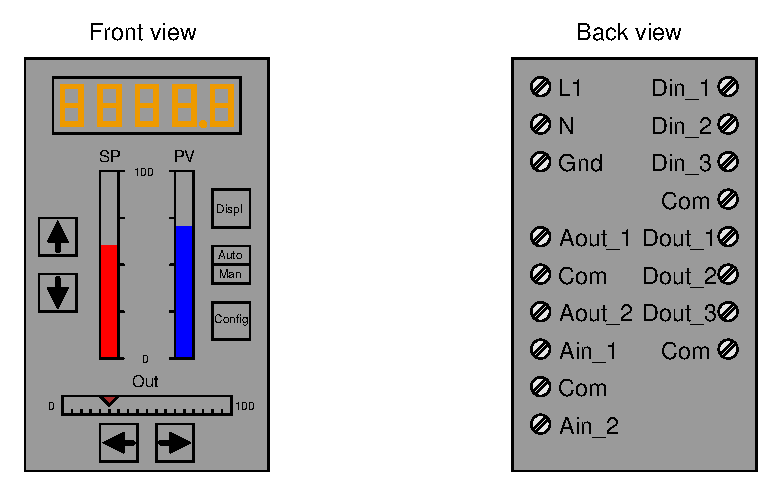
\includegraphics[width=15.5cm]{i02426x01.eps}$$

Distributed control systems (DCS) are quite different.  These systems are designed to control {\it hundreds} or even {\it thousands} of loops.  As such, they are made in a modular fashion so the users can add whatever types of input and output (I/O) capability they need.

Identify the purpose of each type of I/O module listed here, as it might be applied in a DCS.  What I'm looking for here is an educated guess from you, as it may be quite a challenge to actually research these specific I/O types for different distributed control systems:

\begin{itemize}
\item{} AI 1-5 VDC
\vskip 10pt
\item{} AI 4-20 mADC
\vskip 10pt
\item{} AI 4-20 mADC w/ HART
\vskip 10pt
\item{} AO 4-20 mA
\vskip 10pt
\item{} AO w/ HART
\vskip 10pt
\item{} DI 24VDC dry contact
\vskip 10pt
\item{} DI 24VDC isolated
\vskip 10pt
\item{} DI 120VAC isolated
\vskip 10pt
\item{} DO 24VDC high side
\end{itemize}

\underbar{file i02426}
%(END_QUESTION)





%(BEGIN_ANSWER)

\begin{itemize}
\item{} AI 1-5 VDC {\it Analog input, requires external 250 $\Omega$ resistor and loop power supply}
\vskip 10pt
\item{} AI 4-20 mADC {\it Analog input, provides loop power for transmitter with no need for external resistor}
\vskip 10pt
\item{} AI 4-20 mADC w/ HART {\it Analog input, provides loop power and HART communication ability}
\vskip 10pt
\item{} AO 4-20 mA {\it Analog output, drives 4-20 mA DC to device}
\vskip 10pt
\item{} AO w/ HART {\it Analog output, drives 4-20 mA DC to device and provides HART communication ability}
\vskip 10pt
\item{} DI 24VDC dry contact {\it Discrete input, provides power for switch circuit}
\vskip 10pt
\item{} DI 24VDC isolated {\it Discrete input with electrically isolated channels, requires external 24 VDC power source}
\vskip 10pt
\item{} DI 120VAC isolated {\it Discrete input with electrically isolated channels, requires external 120 VAC power source}
\vskip 10pt
\item{} DO 24VDC high side {\it Discrete output, sources 24 VDC to field device when activated}
\end{itemize}

%(END_ANSWER)





%(BEGIN_NOTES)


%INDEX% DCS, I/O: different types

%(END_NOTES)


